\documentclass[12pt]{article}
\usepackage[a4paper, margin=0.75in]{geometry}
\usepackage[document]{ragged2e}
\usepackage{graphicx}
\usepackage{multicol}
\graphicspath{ {./images/} }
\usepackage{enumerate}
\usepackage{framed}
\usepackage{amsmath,amsfonts,amsthm,thmtools,amssymb,mathtools,commath}
\usepackage{physics}
\usepackage{tikz}
\usetikzlibrary{mindmap}
\usepackage{caption}
\usepackage{xcolor}
\usepackage[most]{tcolorbox}
\usepackage{cleveref}


%%%%%%%%%%%%%%%%
%  Definition  %
%%%%%%%%%%%%%%%%
\tcbuselibrary{theorems,skins,hooks}
\newtcbtheorem[number within=subsection]{definition}{Definition}%
{
    % theorem style=definition,
    enhanced,
	before skip=2mm,after skip=2mm, colback=cyan!5,colframe=cyan!80!black,boxrule=0.5mm,
	attach boxed title to top left={xshift=1cm,yshift*=1mm-\tcboxedtitleheight},
	boxed title style={frame code={
					\path[fill=cyan]
					([yshift=-1mm,xshift=-1mm]frame.north west)
					arc[start angle=0,end angle=180,radius=1mm]
					([yshift=-1mm,xshift=1mm]frame.north east)
					arc[start angle=180,end angle=0,radius=1mm];
					\path[left color=cyan!30!black,right color=cyan!30!black,
						middle color=cyan!50!black]
					([xshift=-2mm]frame.north west) -- ([xshift=2mm]frame.north east)
					[rounded corners=1mm]-- ([xshift=1mm,yshift=-1mm]frame.north east)
					-- (frame.south east) -- (frame.south west)
					-- ([xshift=-1mm,yshift=-1mm]frame.north west)
					[sharp corners]-- cycle;
				},interior engine=empty,
		},
	fonttitle=\bfseries,
	title={#2},#1
}{def}


%%%%%%%%%%%%%
%  Theorem  %
%%%%%%%%%%%%%
\tcbuselibrary{theorems,skins,hooks}
\newtcbtheorem[use counter from=definition]{theorem}{Theorem}%
{
    theorem style=plain,
    enhanced,
    colframe=green,
    boxrule=1pt,
    titlerule=0mm,
    toptitle=1mm,
    bottomtitle=1mm,
    fonttitle=\bfseries,
    fontupper=\mdseries\itshape,
    coltitle=green!30!black,
    colbacktitle=cyan!15!white,
    colback=green!10,
    description font=\bfseries\sffamily
}{thrm}


%%%%%%%%%%%%%%
% Corollary  %
%%%%%%%%%%%%%%
 \tcbuselibrary{theorems,skins}
 \newtcbtheorem[use counter from=theorem]{corollary}{Corollary}%
 {
    theorem style=plain,
    enhanced,
    colframe=green,
    frame hidden,
    titlerule=0mm,
    toptitle=1mm,
    bottomtitle=1mm,
    fonttitle=\bfseries,
    fontupper=\mdseries\itshape,
    coltitle=green!30!black,
    colbacktitle=cyan!15!white,
    colback=green!10,
    description font=\bfseries\sffamily
 }{corl}


%%%%%%%%%%%%%
%  Example  %
%%%%%%%%%%%%%
\tcbuselibrary{theorems,skins,hooks}
\newtcbtheorem[number within=section]{example}{Example}%
{
	enhanced,
	breakable,
	colback = gray!5,
	frame hidden,
	boxrule = 0sp,
	borderline west = {2pt}{0pt}{gray},
	sharp corners,
	detach title,
	before upper = \tcbtitle\par\smallskip,
    coltitle=gray!70!black,
	fonttitle = \bfseries\sffamily,
	description font = \mdseries\bfseries
}
{xmp}


%%%%%%%%%%%%%%
%  Exercise  %
%%%%%%%%%%%%%%
\tcbuselibrary{theorems,skins,hooks}
\newtcbtheorem[number within=section]{exercise}{Exercise}%
{
    enhanced,
    breakable,
    colback=black!5,
    colframe=black!30,
    left=0.5em,
    before skip=10pt,
    after skip=10pt,
    boxrule=0pt,
    boxsep=0pt,
    arc=0pt,
    outer arc=0pt,
    borderline west={3pt}{0pt}{black!30},
}{exc}

%%%%%%%%%%
%  Note  %
%%%%%%%%%%
\usetikzlibrary{arrows,calc,shadows.blur}
\tcbuselibrary{skins}
\newtcolorbox{note}[1][]{%
	enhanced jigsaw,
	colback=gray!20!white,%
	colframe=gray!80!black,
	size=small,
	boxrule=1pt,
	title=\textbf{Note:-},
	halign title=flush center,
	coltitle=black,
	breakable,
	drop shadow=black!50!white,
	attach boxed title to top left={xshift=1cm,yshift=-\tcboxedtitleheight/2,yshifttext=-\tcboxedtitleheight/2},
	minipage boxed title=1.5cm,
	boxed title style={%
			colback=white,
			size=fbox,
			boxrule=1pt,
			boxsep=2pt,
			underlay={%
					\coordinate (dotA) at ($(interior.west) + (-0.5pt,0)$);
					\coordinate (dotB) at ($(interior.east) + (0.5pt,0)$);
					\begin{scope}
						\clip (interior.north west) rectangle ([xshift=3ex]interior.east);
						\filldraw [white, blur shadow={shadow opacity=60, shadow yshift=-.75ex}, rounded corners=2pt] (interior.north west) rectangle (interior.south east);
					\end{scope}
					\begin{scope}[gray!80!black]
						\fill (dotA) circle (2pt);
						\fill (dotB) circle (2pt);
					\end{scope}
				},
		},
	#1,
}


\title{
    \textbf{Experiment 12} \\
    \textbf{Experiment on Band Pass Filter} \\
}

\author{
    Turja Roy \\
    ID: 2108052
}
\date{}

\begin{document}
\maketitle

\section{Objective}
\begin{enumerate}
    \item To determine the Band Pass Filter frequency response of an RC circuit. 
    \item To measure the cut off frequency and observe the attenuation rate. 
    \item To compare the graph of simulation data and practical data.
\end{enumerate}

\section{Apparatus}
\begin{multicols}{2}
    \begin{enumerate}
        \item Resistors
        \item Capacitors
        \item Oscilloscope
        \item Breadboard
    \end{enumerate}
    \columnbreak
    \begin{enumerate}
        \item Wires
        \item Function Generator
        \item DC Power Supply
        \item Multimeter
    \end{enumerate}
\end{multicols}

\section{Circuit Diagram}
\begin{figure}[h]
    \centering
    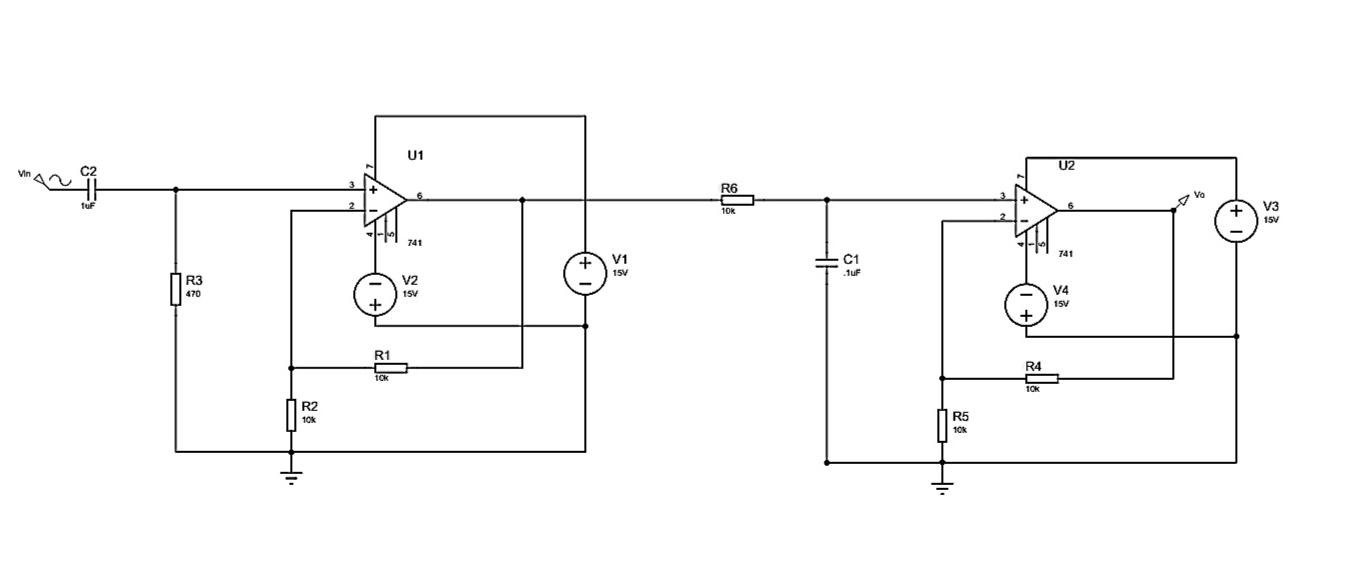
\includegraphics[width=0.9\textwidth]{BPF.png}
    \caption{Band Pass Filter RC Circuit}
\end{figure}

\section{Result Analysis}
The circuit configuration on Figure 1 entails an active band pass filter where an active high-pass filter(HPF) and an active low-pass filter (LPF) are connected in series via a resistor R6. This arrangement facilitates the transmission of signals within a specified frequency range while attenuating both low and highfrequency components. The resistor R6 acts as a coupling element, regulating the flow of signals between the filters.

\subsection{Data Table}

Table 1 represents the experimental output data. The input and output voltage Vout are in volts. The voltage gain is calculated in decibel(dB) using the equation
\[
    A_v = 20 \log \left( \frac{V_{out}}{V_{in}} \right)
\] 

\begin{table}[h!]
    \centering
    \caption{Practical Data of Band Pass Filter}
    \begin{tabular}{rrrr}
        \hline
        Vin &  Vout &  frequency &         Av \\
        \hline
        1 & 0.045 &        0.1 & -26.935750 \\
        1 & 0.063 &        5.0 & -24.013189 \\
        1 & 0.072 &        6.0 & -22.853350 \\
        1 & 0.082 &        7.0 & -21.723723 \\
        1 & 0.098 &        8.0 & -20.175478 \\
        1 & 0.104 &        9.0 & -19.659333 \\
        1 & 0.117 &       10.0 & -18.636283 \\
        1 & 0.127 &       11.0 & -17.923926 \\
        1 & 0.130 &       12.0 & -17.721133 \\
        1 & 0.133 &       13.0 & -17.522967 \\
        1 & 0.145 &       14.0 & -16.772640 \\
        1 & 0.166 &       15.0 & -15.597838 \\
        1 & 0.187 &       16.0 & -14.563168 \\
        1 & 0.187 &       17.0 & -14.563168 \\
        1 & 0.187 &       18.0 & -14.563168 \\
        1 & 0.187 &       19.0 & -14.563168 \\
        1 & 0.192 &       20.0 & -14.333975 \\
        1 & 0.182 &       21.0 & -14.798572 \\
        1 & 0.182 &       22.0 & -14.798572 \\
        1 & 0.182 &       23.0 & -14.798572 \\
        1 & 0.179 &       24.0 & -14.942939 \\
        1 & 0.176 &       25.0 & -15.089747 \\
        1 & 0.176 &       26.0 & -15.089747 \\
        1 & 0.176 &       27.0 & -15.089747 \\
        1 & 0.175 &       30.0 & -15.139239 \\
        1 & 0.175 &       35.0 & -15.139239 \\
        1 & 0.160 &       60.0 & -15.917600 \\
        1 & 0.159 &       80.0 & -15.972058 \\
        1 & 0.152 &      150.0 & -16.363128 \\
        1 & 0.062 &      400.0 & -24.152166 \\
        1 & 0.045 &      550.0 & -26.935750 \\
        \hline
    \end{tabular}
\end{table}

\newpage
\subsection{Graph}

\begin{figure}[h]
    \centering
    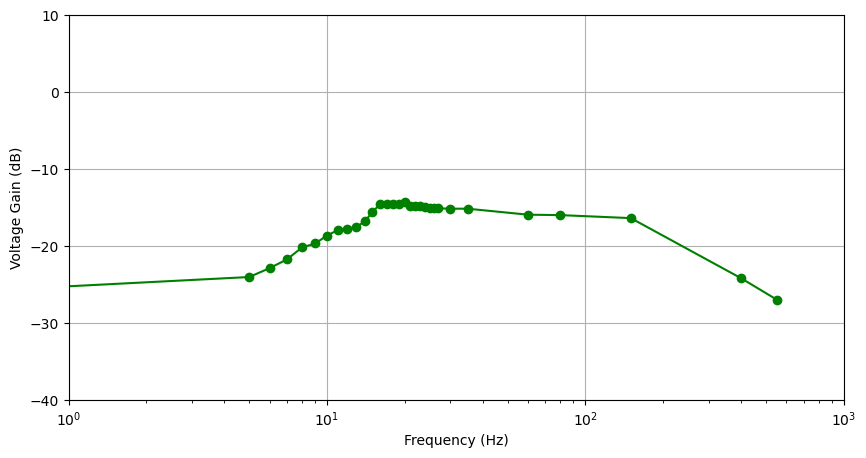
\includegraphics[width=0.8\textwidth]{BPF_Graph.png}
    \caption{Frequency Response of Band Pass Filter}
\end{figure}

The graph in Figure 2 shows the frequency response of the band pass filter. The gain is highest at a mid-range frequency. The filter blocks higher frequencies and passes lower frequencies. The filter looks like a high pass filter after increasing the frequency and a low pass filter after decreasing the frequency. The condition of the band pass filter is observed.

\section{Discussion}

In this experiment, the band pass filter frequency response of an RC circuit is determined. The cut off frequency is observed at 15 Hz. The attenuation rate is observed to be -20 dB/decade. The graph of simulation data and practical data is compared. The graph shows the frequency response of the band pass filter. The gain is highest at a mid-range frequency. The filter blocks higher frequencies and passes lower frequencies. The filter looks like a high pass filter after increasing the frequency and a low pass filter after decreasing the frequency. The condition of the band pass filter is observed.

\end{document}

